\documentclass[11pt,a4paper]{article}
\usepackage[utf8]{inputenc}
\usepackage[T1]{fontenc}
\usepackage[brazil]{babel}
\usepackage[margin=2.3cm]{geometry}
\usepackage{booktabs}
\usepackage{amsmath,amssymb}
\usepackage{caption}
\usepackage{graphicx}
\usepackage{setspace}
\usepackage{enumitem}
\usepackage{xcolor}
\usepackage[hidelinks]{hyperref}
\graphicspath{{docs/}}
\definecolor{azul}{RGB}{20,60,110}
\definecolor{verde}{RGB}{20,110,70}
\definecolor{vermelho}{RGB}{150,30,30}
\newcommand{\pergunta}[1]{\par\vspace{4pt}\noindent\textbf{\color{azul}A pergunta:} #1\par\vspace{2pt}}
\newcommand{\analogia}[1]{\par\vspace{4pt}\noindent\textbf{\color{verde}Pensa assim:} #1\par\vspace{2pt}}
\newcommand{\exemplo}[0]{\par\vspace{4pt}\noindent\textbf{\color{vermelho}Exemplo com números:}\ }
\newcommand{\aha}[1]{\par\vspace{4pt}\noindent\textbf{\color{vermelho}O momento "ahá":} #1\par\vspace{2pt}}
\newcommand{\noprojeto}[0]{\par\vspace{4pt}\noindent\textbf{No seu projeto:}\ }
\graphicspath{{docs/}}
\emergencystretch=2.5em
\setstretch{1.15}
\captionsetup{font=small,labelsep=colon}
\setcounter{tocdepth}{2}

\title{\textbf{Explicação}\\[8pt]
\Large O projeto inteiro, devagar, do jeito que faz sentido de verdade\\[4pt]
\normalsize Peso de VALE3 nos fundos do grupo Itaú --- guia completo, com analogias,\\
exemplos numéricos passo a passo e a resposta de ``o quê, por quê e como''\\
para cada peça do trabalho}
\author{João Paulo Zangrandi (FGV--EESP)\\[2pt]\small documento de apoio ao \texttt{tcc I.pdf}; escrito para ler antes ou junto com ele}
\date{}

\begin{document}
\maketitle

\begin{abstract}
\noindent Este documento existe para uma única finalidade: explicar \emph{tudo} que acontece no
projeto, do começo ao fim, sem pressa e sem pular etapas. Cada método aparece na mesma ordem:
primeiro a pergunta que ele responde, depois uma analogia do dia a dia, depois um exemplo com
números inventados (mas realistas) que você pode conferir na calculadora, e só então o que
aconteceu de fato nos seus dados. Nada aqui substitui o \texttt{tcc I.pdf} --- é o texto que fica
do lado, para consultar sempre que uma passagem dele parecer rápida demais.
\end{abstract}

\newpage
\tableofcontents
\newpage

% ======================================================================
\section{O mapa da história inteira, antes de qualquer detalhe}

O projeto conta uma história em duas partes, e vale muito a pena ter essa história inteira na
cabeça antes de entrar em qualquer fórmula.

\textbf{Parte 1 --- Explicar.} Você tem 307 fundos do grupo Itaú, ao longo de 72 meses
(2016--2021), e para cada um sabe quanto de VALE3 ele carrega na carteira (o \emph{peso}). Você
também sabe algumas características de cada fundo: tamanho, número de cotistas, se é um fundo
que investe em outros fundos (FIC) ou direto em ações, e quanto ele captou ou resgatou naquele
mês. A primeira pergunta do trabalho é: \textbf{essas características explicam o peso?} A
resposta, resumidamente, é sim --- fundos maiores carregam menos VALE3 em peso, fundos com mais
cotistas carregam mais, fundos de cotas carregam menos.

\textbf{Parte 2 --- Prever.} Sabendo que as características explicam o peso, a segunda pergunta
é: \textbf{isso ajuda a prever o peso do mês seguinte?} Aqui a resposta é mais surpreendente:
não muito. O peso de cada fundo é tão parecido de um mês para o outro que simplesmente
``repetir o valor do mês passado'' é uma previsão difícil de bater. O resto do trabalho
investiga \emph{por que} isso acontece e se existe, ainda assim, algum sinal de que os fundos
caminham devagar em direção a um alvo definido pelas características.

Este documento segue essa mesma ordem: primeiro as ferramentas da Parte 1 (Fama--MacBeth,
Newey--West, o modelo logístico), depois as da Parte 2 (dinâmica do fator, teste de
Dickey--Fuller, filtro de Kalman, previsão, a margem extensiva de ter ou não ter a ação), e por
fim a peça mais elaborada do trabalho, o modelo de ajuste parcial --- com os quatro métodos de
estimação, a correção do erro-padrão por efeito de tempo, e o teste de Diebold--Mariano --- que
tenta reconciliar as duas partes. As extensões (fatores NEFIN, beta do fundo, e a generalização
para outras ações) fecham o documento.

% ======================================================================
\section{Os dados: o que existe, e por que cada tratamento foi feito}

\subsection{As quatro fontes de informação}

\begin{itemize}[topsep=2pt,itemsep=3pt]
\item \textbf{A composição das carteiras (CONS, CVM)} --- é de onde vem a variável mais
importante do trabalho: quanto de VALE3 cada fundo tem, mês a mês, em fração da carteira (o
peso). Uma descoberta útil desta versão: esse arquivo já vem filtrado pela CVM só para
\emph{ações}, não é a carteira inteira do fundo (que teria também renda fixa, por exemplo).
\item \textbf{A série histórica dos fundos (SH, CVM)} --- de onde vêm as características: o
patrimônio do fundo, quantos cotistas ele tem, e se o nome dele indica que é um fundo de cotas
(FIC).
\item \textbf{O Informe Diário (CVM)} --- de onde vem a captação líquida (quanto entrou menos
quanto saiu do fundo naquele mês). Precisou de uma fonte à parte porque a SH só registra a
captação bruta, sem os resgates.
\item \textbf{Cotações de mercado (Yahoo Finance)} --- de onde vêm o preço e o beta de VALE3,
conferidos contra a fonte oficial da B3.
\end{itemize}

\subsection{Por que tanto cuidado de limpeza}

\pergunta{Por que não simplesmente juntar as bases e rodar a regressão?}

\analogia{Imagina que você está montando um quebra-cabeça com peças de duas caixas diferentes.
Antes de encaixar qualquer peça, você confere se elas realmente são do mesmo quebra-cabeça
(mesma data, mesmo fundo) e se não tem peça duplicada ou triplicada por engano. Só depois disso
faz sentido começar a montar a imagem.}

\noprojeto\ cada linha da base de composição (CONS) precisou ser casada com a linha certa da
série histórica (SH) --- pelo \emph{dia exato}, porque a SH é diária e a CONS é mensal. Linhas
duplicadas (a CVM às vezes repete uma linha por engano) foram removidas. Pesos negativos (um
resíduo contábil sem sentido de participação de carteira) foram descartados. E, numa correção
recente, descobrimos que uma mesma ação pode aparecer em até cinco linhas diferentes na base
bruta, dependendo do tipo de custódia (posição direta, ação emprestada, direito de compra de
ações novas) --- sem isso ser cinco ações diferentes. Filtramos para manter só a posição direta,
a mesma convenção usada para VALE3 desde o início.

\subsection{Por que o peso, e não o valor em reais}

\pergunta{Por que medir ``quanto de VALE3'' como uma fração da carteira (peso), em vez de em
reais?}

\analogia{Se você quer comparar o quanto duas pessoas de renda muito diferente gastam com
lazer, comparar em reais engana --- R\$~500 é muito para quem ganha R\$~2.000 e pouco para quem
ganha R\$~50.000. Comparar em \emph{porcentagem da renda} resolve isso. O peso faz o mesmo
serviço para fundos de tamanhos muito diferentes.}

O peso tem uma vantagem e uma complicação. A vantagem: é sempre um número entre 0\% e 100\%,
comparável entre um fundo pequeno e um fundo gigante. A complicação: exatamente por ser limitado
entre 0 e 1, uma regressão linear comum (uma reta) pode devolver previsões sem sentido --- um
peso negativo, ou maior que 100\%. É essa complicação que motiva a curva logística, explicada na
próxima seção.

% ======================================================================
\section{A curva em S (logit): por que existe, e como funciona por dentro}
\label{sec:curva}

\pergunta{Como transformar uma combinação de características (tamanho, cotistas, tipo de fundo)
num número que \emph{sempre} fica entre 0\% e 100\%, não importa quão extremas sejam as
características?}

\subsection{Por que uma reta não serve}

Se você tentasse escrever ``peso = 4\% + (ajuste por tamanho) + (ajuste por cotistas) + \dots''
como uma soma direta, nada impede o resultado de dar, por exemplo, $-3\%$ ou $115\%$ --- números
sem sentido para uma fração de carteira. Precisamos de uma ``máquina'' que aceite qualquer
combinação de entrada e sempre devolva algo dentro do intervalo válido.

\subsection{A curva em S, sem fórmula ainda}

Existe uma curva com formato de S deitado que faz exatamente isso. O comportamento dela, em
palavras, antes de qualquer conta:

\begin{itemize}[topsep=2pt,itemsep=2pt]
\item Se você entra com um número \textbf{bem negativo}, ela devolve algo \textbf{bem perto de
0\%} (nunca chega a tocar em 0\%, mas fica bem próximo).
\item Se você entra com \textbf{zero}, ela devolve exatamente \textbf{50\%}.
\item Se você entra com um número \textbf{bem positivo}, ela devolve algo \textbf{bem perto de
100\%}.
\end{itemize}

\analogia{É como um amortecedor de carro: não importa o tamanho do buraco na estrada (a entrada
pode ser qualquer número), a suspensão sempre entrega um movimento dentro de um limite físico
(a saída fica sempre dentro de uma faixa).}

\subsection{A fórmula, com números pequenos para você ver funcionando}

$$g(z) = \frac{1}{1+e^{-z}}$$

$z$ é o número que você coloca na máquina; $e$ é só uma constante ($\approx 2{,}718$). Testando:

\begin{center}\small
\begin{tabular}{@{}rrl@{}}
\toprule
Entrada ($z$) & Cálculo & Saída ($g(z)$) \\
\midrule
$0$ & $\frac{1}{1+e^{0}}=\frac{1}{1+1}$ & $0{,}500 \to 50{,}0\%$ \\
$-3$ & $\frac{1}{1+e^{3}}=\frac{1}{1+20{,}1}$ & $0{,}047 \to 4{,}7\%$ \\
$+3$ & $\frac{1}{1+e^{-3}}=\frac{1}{1+0{,}05}$ & $0{,}953 \to 95{,}3\%$ \\
\bottomrule
\end{tabular}
\end{center}

Repare que $-3$ e $+3$ deram resultados espelhados (4,7\% e 95,3\%, que somam 100\%) --- a curva
é simétrica em torno do 50\%.

\subsection{De onde vem o ``$z$'' que entra nessa máquina}

$z$ não é um número solto --- é uma \textbf{nota combinada}, montada somando pontos a favor e
contra, um por característica do fundo:

$$z = \underbrace{-3{,}18}_{\text{nota base}} \;-\; \underbrace{0{,}18\times(\text{tamanho})}_{\text{penalidade}} \;+\; \underbrace{0{,}30\times(\text{cotistas})}_{\text{bônus}} \;-\; \underbrace{0{,}55\times(\text{é FIC?})}_{\text{penalidade}}$$

\analogia{É a mesma lógica de um score de crédito: o banco combina renda, histórico de
pagamento e dívidas --- coisas em escalas completamente diferentes --- numa nota única. Aqui a
nota combina tamanho, cotistas e tipo de fundo numa única nota que resume o ``perfil'' daquele
fundo para prever o peso.}

\subsection{Por que as características entram numa escala especial (padronização)}

\pergunta{Por que não somar direto o tamanho em reais com o número de cotistas?}

Tamanho é medido em reais (pode ser R\$~70 milhões); cotistas é medido em pessoas (pode ser
100). Somar $70.000.000 + 100$ diretamente não faz sentido --- o tamanho dominaria tudo. A
solução é colocar as duas na mesma régua antes de somar: em vez do valor bruto, você usa
``quantos degraus acima ou abaixo da média esse fundo está''. Um fundo exatamente na média vale
$0$ nessa régua; um fundo bem maior que a média vale $1$, $2$, ou mais; um fundo bem menor vale
negativo. \noprojeto\ isso aparece como $z(\ln PL)$ e $z(\ln Cot)$ na equação (3) do
\texttt{tcc I.pdf}, Seção 3.2 --- o texto descreve em palavras (``entram centradas e divididas
pelo desvio padrão''), mas não escreve a fórmula por extenso; ela é
$z(x) = \frac{x - \text{média de }x}{\text{desvio-padrão de }x}$.

\subsection{Juntando tudo: um exemplo completo, com um fundo de verdade}

\exemplo\ um fundo \textbf{grande} (1 degrau acima da média em tamanho) e que \textbf{é FIC}
(cotistas na média). Usando os coeficientes reais de janeiro de 2020:

$$z = -3{,}18 - 0{,}18\times 1 + 0{,}30\times 0 - 0{,}55\times 1 = -3{,}91$$
$$w^* = g(-3{,}91) = \frac{1}{1+e^{3{,}91}} \approx \frac{1}{1+49{,}9} \approx 2{,}0\%$$

Esse $2{,}0\%$ é o \textbf{peso desejado} (o alvo) desse fundo naquele mês --- não uma ordem, é
uma comparação estatística: ``fundos com esse perfil, naquele mês, costumavam ter cerca de
2,0\%''.

\noprojeto\ o \texttt{tcc I.pdf} não mostra esse exemplo de um mês isolado --- ele mostra, na
\textbf{Tabela 3, Seção 4.2}, a \emph{média} dos 72 meses desses mesmos coeficientes:
Intercepto$=-3{,}380$, $\ln$(patrimônio)$=-0{,}339$, $\ln$(cotistas)$=0{,}469$, Fundo de
cotas$=-0{,}732$ --- bem parecidos com os do exemplo, porque os coeficientes mensais são
estáveis ao longo do tempo (Seção 4.5).

\subsection{Por que essa forma logística é melhor que uma reta, na prática}

\noprojeto\ a versão linear (uma reta simples, sem a curva em S) foi testada em paralelo e gerou
previsões de peso \textbf{fora do intervalo $[0,1]$ em 2,51\% das observações} --- pesos
negativos, sem sentido. A versão logística nunca faz isso, por construção. Além disso, o ajuste
melhora ligeiramente (um indicador parecido com $R^2$ sobe de $0{,}152$ para $0{,}165$).

\subsection{O efeito parcial médio: traduzindo a nota de volta para pontos percentuais}

\pergunta{O coeficiente $-0{,}339$ do tamanho está na escala de ``nota'' ($z$), não em pontos
percentuais de peso. Como traduzir de volta?}

Para variáveis contínuas (tamanho, cotistas), a tradução usa a inclinação da curva no ponto
médio: multiplica o coeficiente por $g(1-g)$ (a inclinação da curva em S naquele ponto).
\noprojeto\ isso dá, por exemplo, $-0{,}68$ ponto percentual para tamanho, $+1{,}06$ para
cotistas --- \textbf{Tabela 3, Seção 4.2, coluna ``Ef. parcial (p.p.)''}.

\subsubsection*{O cuidado especial com a dummy FIC}

\pergunta{Por que ``ser FIC ou não'' precisa de um cálculo diferente das outras variáveis?}

\analogia{A tradução por inclinação (usada para tamanho e cotistas) funciona bem para
\emph{pequenos passos} ao longo da curva --- como usar a velocidade instantânea de um carro para
estimar a distância percorrida num segundo. Mas ``ser FIC ou não'' não é um passo pequeno --- é
um salto completo entre dois estados (é ou não é), como comparar a posição do carro no início e
no fim de uma freada brusca, não só a velocidade num instante.}

O cálculo certo para uma dummy é a \textbf{diferença discreta}: calcular o peso previsto
fingindo que o fundo \emph{é} FIC, calcular de novo fingindo que \emph{não é}, e subtrair de
verdade.

\exemplo\ para um fundo típico, em janeiro de 2020: peso previsto com FIC$=0$ é $4{,}01\%$; peso
previsto com FIC$=1$ é $2{,}34\%$. A diferença de verdade é $2{,}34-4{,}01=-1{,}67$ pontos
percentuais. O método da inclinação (usado antes de uma correção) dava só $-1{,}52$ --- porque o
coeficiente de FIC é grande, o salto entre os dois estados é longo, e a reta tangente usada pelo
método da inclinação não acompanha a curvatura da curva em S ao longo de todo esse salto.

\noprojeto\ agregando os 72 meses, essa diferença sistemática vira $-1{,}60$ (derivada, método
antigo) contra $-1{,}94$ (diferença discreta, método corrigido) --- quase 20\% de diferença,
\textbf{Tabela 3, Seção 4.2}, nota de rodapé.

% ======================================================================
\section{Fama--MacBeth: por que rodar 72 regressões separadas}
\label{sec:fm}

\pergunta{Por que não empilhar todos os fundos de todos os meses numa regressão só?}

\subsection{O problema que motiva o método}

Fundos do mesmo mês tendem a se mover juntos --- mesma gestora, mesmas condições de mercado
naquele momento. Essa ``dança em grupo'' cria uma correlação entre os erros da regressão que é
difícil de medir diretamente (imagine ter que estimar o quanto cada um dos 150 fundos de um mês
se correlaciona com cada um dos outros 149 --- um número gigante de relações).

\subsection{A solução, em duas etapas}

\textbf{Etapa 1:} em vez de uma regressão gigante, você roda \textbf{uma regressão por mês},
usando só os fundos daquele mês específico. Isso gera 72 ``fotos'' separadas, uma por mês --- 72
vetores de coeficientes $\widehat\theta_1, \widehat\theta_2, \dots, \widehat\theta_{72}$.

\textbf{Etapa 2:} depois de ter as 72 fotos, você simplesmente tira a \textbf{média} de cada
coeficiente ao longo dos 72 meses, e calcula o erro-padrão a partir de \textbf{quanto esses 72
valores variam entre si}.

\analogia{É como perguntar ``qual é a altura média das pessoas de uma cidade'' medindo um bairro
de cada vez, em vez de tentar juntar todo mundo numa fila só. No fim, você tira a média dos
resultados dos bairros --- e a variação entre os bairros já te conta, sozinha, o quanto confiar
nessa média, sem precisar saber exatamente como as pessoas de cada bairro se parecem entre si.}

\subsection{Por que isso é inteligente}

Cada ``foto'' mensal ($\widehat\theta_t$) já é, sozinha, uma função de \textbf{todos} os dados
daquele mês. Então qualquer ``dança em grupo'' que exista dentro daquele mês já está embutida em
quanto aquela foto varia de mês para mês. Você não precisa modelar a correlação entre fundos
diretamente --- ela aparece, de graça, na dispersão da série de 72 fotos.

\subsection{A hipótese que precisa valer (e que falha no seu caso)}

O truque só funciona se as 72 fotos forem \textbf{independentes umas das outras} --- o
coeficiente de fevereiro não pode ``carregar'' informação de janeiro. \noprojeto\ isso falha:
a correlação de um mês para o próximo, nos seus dados, é de $0{,}70$ a $0{,}84$ --- longe de
zero. Isso é corrigido pelo Newey--West, explicado a seguir.

\subsection{O resultado, no seu projeto}

\begin{center}\small
\begin{tabular}{@{}lrr@{}}
\toprule
Coeficiente & Média dos 72 meses & Est. $t$ (corrigida) \\
\midrule
$\ln$(patrimônio) por d.p. & $-0{,}0068$ & $-11{,}3$ \\
$\ln$(cotistas) por d.p. & $+0{,}0109$ & $10{,}9$ \\
Fundo de cotas & $-0{,}0170$ & $-11{,}1$ \\
\bottomrule
\end{tabular}
\end{center}

$\Rightarrow$ \textbf{Tabela 2, Seção 4.1} do \texttt{tcc I.pdf}.

% ======================================================================
\section{Newey--West: por que o erro-padrão simples engana}
\label{sec:nw}

\pergunta{Por que não usar a fórmula clássica de erro-padrão (desvio-padrão da série dividido
pela raiz de 72)?}

\analogia{Imagine perguntar a opinião de 72 pessoas sobre um filme, mas 60 delas são amigas
próximas que sempre concordam entre si (porque conversaram antes de responder). Se você tratar
as 72 respostas como 72 opiniões totalmente independentes, você vai superestimar o quanto sabe
sobre a opinião real da população --- na prática, você tem muito menos que 72 ``vozes''
realmente distintas, porque boa parte delas está só repetindo a opinião das outras.}

Os 72 coeficientes mensais são parecidos com essas 72 pessoas: como se correlacionam de $0{,}70$
a $0{,}84$ de um mês para o outro, tratar os 72 como 72 informações totalmente novas e
independentes \textbf{superestima a precisão} da média --- os erros-padrão saem pequenos demais,
e as estatísticas $t$ saem grandes demais, dando uma falsa sensação de certeza.

\subsection{A correção}

O Newey--West soma não só a variância de cada mês sozinho, mas também as ``covariâncias'' entre
meses vizinhos (o quanto um mês se parece com o mês seguinte, dois meses depois, etc.), com um
peso que diminui quanto mais distante a defasagem. \noprojeto\ o efeito prático foi multiplicar
os erros-padrão por $1{,}7$ a $1{,}8$ --- as estatísticas $t$ caíram de valores em torno de $19$
a $21$ para valores em torno de $11$. As conclusões (todas as características são
significativas) sobrevivem, mas os números ``bonitos demais'' de antes eram uma ilusão de
precisão. $\Rightarrow$ \textbf{Seção 3.3 e Tabela 2, Seção 4.1}.

% ======================================================================
\section{A dinâmica do fator: os coeficientes mudam de mês para mês, e o filtro de Kalman}
\label{sec:kalman}

\subsection{O que a Etapa 1 do Fama--MacBeth já te deu, sem você perceber}

Antes mesmo de calcular a média (Etapa 2), você já tinha 72 números separados --- uma
\textbf{série temporal} de coeficientes. É essa série, e só ela, que alimenta tudo que vem
nesta seção. O filtro de Kalman nunca olha para os dados originais de fundo por fundo --- só
para essa sequência já resumida mês a mês.

\subsection{Por que essa série é ``barulhenta''}

Cada coeficiente mensal $\widehat\theta_t$ não é o valor ``verdadeiro'' daquele mês --- é o
valor verdadeiro mais um erro de amostragem (cada mês usa uma amostra diferente de
$\sim$150 fundos, e amostra finita sempre erra um pouco):

$$\widehat\theta_t = \underbrace{\mu_t}_{\text{fator verdadeiro}} + \underbrace{\varepsilon_t}_{\text{ruído daquele mês}}$$

\subsection{Antes do Kalman: como saber se a série ``sempre volta ao mesmo lugar'' ou ``pode se
afastar para sempre''? O teste de Dickey--Fuller}
\label{sec:df}

\pergunta{Antes de decidir como prever os coeficientes, precisamos saber: eles têm um ``centro de
gravidade'' para onde sempre voltam, ou podem se afastar dele permanentemente?}

\analogia{Pensa numa bolinha de gude. Se você solta ela dentro de uma tigela funda, não importa
de onde você solte, ela sempre rola de volta para o fundo --- existe um ``centro de gravidade''.
Isso é \textbf{reversão à média}. Agora imagina soltar a mesma bolinha numa mesa completamente
plana e sem atrito: ela fica exatamente onde parou, e qualquer empurrãozinho a leva para um lugar
novo, \textbf{permanentemente} --- não existe centro de gravidade nenhum. Isso é \textbf{passeio
aleatório} (também chamado de ``raiz unitária'').}

\textbf{Por que isso importa aqui:} se os coeficientes $\theta_t$ fossem um passeio aleatório
puro, a melhor previsão de amanhã seria simplesmente o valor de hoje (não haveria nenhum ``centro''
para o qual a série tende a voltar). Se eles revertem à média, faz sentido usar um modelo (como o
Kalman) que capture essa tendência de retorno.

\subsubsection*{Como o teste funciona, por dentro}

A ideia é reescrever a pergunta ``a série reverte à média?'' como uma regressão: a \textbf{mudança}
da série de um mês para o outro é explicada por \textbf{onde a série estava} no mês anterior.

\begin{itemize}[topsep=2pt,itemsep=2pt]
\item Se o coeficiente dessa relação for \textbf{zero}: a mudança de amanhã não depende de onde
você está hoje --- é a mesa plana, passeio aleatório.
\item Se for \textbf{negativo} (e claramente diferente de zero): quando a série está longe do
centro, ela tende a se mover de volta --- é a tigela, reversão à média.
\end{itemize}

\subsubsection*{A pegadinha: por que não usar a tabela de significância comum}

\pergunta{Por que esse teste usa um valor crítico diferente ($-2{,}9$) em vez do $-1{,}65$ ou
$-1{,}96$ de um teste comum?}

Aqui está o detalhe sutil: \textbf{debaixo da hipótese que está sendo testada} (passeio
aleatório), a própria variável usada para explicar a mudança não tem ``chão'' --- ela pode vagar
para qualquer lugar, sem limite. Isso quebra uma suposição matemática que os testes comuns
precisam (que a variável explicativa se comporte de um jeito ``bem-comportado''), e a distribuição
da estatística do teste fica deslocada --- por isso o valor crítico é mais exigente
($\approx-2{,}9$ a 5\% de significância, não $-1{,}65$).

\noprojeto\ rodando esse teste nas 5 séries de coeficientes (72 meses cada), quatro delas
rejeitam passeio aleatório puro --- intercepto, tamanho e FIC claramente revertem à média (o teste
dá valores mais negativos que $-2{,}9$); cotistas fica bem no limite ($-2{,}70$, quase lá, mas
tecnicamente não rejeita a 5\%); fluxo é a menos persistente de todas, quase ruído puro. Esse
resultado --- as séries revertem, mas devagar --- é exatamente a evidência que justifica usar o
filtro de Kalman em vez de tratar a série como puro ruído ou puro passeio aleatório.
$\Rightarrow$ \textbf{Seção 4.5, Tabela 5, ``Dinâmica dos coeficientes''.}

\subsection{Duas formas diferentes de lidar com essa série barulhenta}

\textbf{Caminho 1 (Fama--MacBeth, Etapa 2):} tira uma média única dos 72 valores --- ótimo para
``em média, ao longo de todo o período, essa característica importa?'', mas descarta a ordem
temporal.

\textbf{Caminho 2 (filtro de Kalman):} percorre a série mês a mês, tentando reconstruir a
trajetória ``verdadeira'' que está por trás dos 72 valores ruidosos, permitindo que ela realmente
se mova ao longo do tempo.

\analogia{Pensa nos 72 $\widehat\theta_t$ como 72 fotos de algo que se move devagar, cada foto um
pouco embaçada. O Fama--MacBeth (Caminho 1) sobrepõe as 72 fotos numa imagem composta só --- boa
para dizer ``na média, foi assim'', mas perde o movimento. O Kalman (Caminho 2) monta um
\emph{vídeo}: reconstrói a trajetória suave mais provável por trás daquela sequência de fotos
embaçadas.}

\subsection{Como o filtro decide quanto confiar em cada mês novo}

O filtro estima duas variâncias separadas: $Q$ (o quanto o fator realmente se move de mês para
mês) e $R$ (o quanto cada mês individual erra por causa da amostra). A partir delas, calcula um
\textbf{ganho} $K_t \in (0,1)$ que decide, mês a mês, o quanto ``acreditar'' no valor novo:

\begin{itemize}[topsep=2pt,itemsep=2pt]
\item Se o ruído de medida domina ($R \gg Q$): $K \to 0$, o filtro quase ignora o mês novo ---
vira uma média longa.
\item Se o estado se move muito ($Q \gg R$): $K \to 1$, o filtro quase copia o valor novo --- vira
``repetir o último valor''.
\end{itemize}

\noprojeto\ por que faz sentido usar Kalman em vez de só a média: a autocorrelação de $0{,}70$ a
$0{,}84$ (Seção~\ref{sec:fm}) mostra que a série \textbf{não é só ruído em torno de uma média
fixa} --- ela realmente se move, com uma reconfiguração visível em torno de 2018. Se fosse só
ruído, a média já seria a melhor descrição possível.

% ======================================================================
\section{Previsão: os quatro modelos e por que a ingênua vence}
\label{sec:previsao}

\pergunta{As características explicam bem o peso contemporâneo --- será que também ajudam a
prever o peso do mês seguinte?}

Quatro modelos competem, todos avaliados fora da amostra (só com informação disponível até o
momento da previsão):

\begin{itemize}[topsep=2pt,itemsep=3pt]
\item \textbf{M0 (ingênua):} $\widehat w_{t+1} = w_t$ --- simplesmente repete o último peso. É a
régua contra a qual todos os outros precisam ganhar.
\item \textbf{M1 (efeito fixo):} $\widehat w_{t+1} = \bar w_i$ --- usa a média histórica \emph{do
próprio fundo}. Testa se o peso reverte a um nível característico daquele fundo.
\item \textbf{M2 (efeito fixo + Kalman):} soma ao nível do fundo o desvio que as características
sugerem, usando o fator suavizado pelo Kalman.
\item \textbf{M3 (variação):} prevê diretamente a \emph{mudança} do peso, usando o fluxo e outras
características.
\end{itemize}

\subsection{O resultado, e por que ele é revelador}

\begin{center}\small
\begin{tabular}{@{}lrrrr@{}}
\toprule
Universo & M0 ingênua & M1 efeito fixo & M2 EF+Kalman & M3 variação \\
\midrule
Todos, $h=1$ mês & $\mathbf{0{,}0156}$ & $0{,}0240$ & $0{,}0255$ & $0{,}0156$ \\
\bottomrule
\end{tabular}
\end{center}
$\Rightarrow$ \textbf{Tabela 6, Seção 4.6} (RMSE, menor é melhor).

\textbf{A ingênua vence todos.} O resultado mais revelador é \textbf{M1 perder de M0}: se
existisse reversão à média histórica do próprio fundo, M1 venceria M0. Ele não vence ---
significa que \textbf{não há reversão detectável ao nível do fundo no curto prazo}: o peso se
comporta quase como um \emph{martingale} (um processo em que a melhor previsão do amanhã é
simplesmente o valor de hoje, sem nenhuma tendência de retorno a média nenhuma). M3 empatar com
M0 diz que nem o fluxo antecipa mudanças de peso.

\analogia{É como tentar prever se vai chover amanhã usando ``a média histórica de chuva desse
mês'' contra ``choveu ou não choveu hoje''. Se ``choveu hoje'' prevê melhor que a média
histórica, isso diz que o clima tem inércia de curto prazo forte --- é basicamente o que
acontece aqui com o peso das carteiras.}

% ======================================================================
\section{A margem extensiva: antes de ``quanto'', existe ``tem ou não tem''}
\label{sec:margens}

\pergunta{Até agora, olhamos só fundos que \emph{já têm} VALE3, perguntando ``quanto''. Mas
existe uma pergunta anterior a essa: o fundo tem VALE3 na carteira ou não?}

\analogia{É a diferença entre perguntar ``quanto alguém gasta com viagens'' (só faz sentido
perguntar para quem viaja) e perguntar ``essa pessoa viaja ou não'' (pergunta que vale para todo
mundo, inclusive quem nunca viajou na vida). A primeira pergunta é a \textbf{margem intensiva}
(quanto, condicional a ter); a segunda é a \textbf{margem extensiva} (ter ou não).}

\subsection{Como se monta essa análise}

Até aqui, a amostra só incluía fundos que detêm VALE3. Para estudar a margem extensiva, é preciso
um painel diferente: \textbf{todos} os fundos de ações do Itaú, inclusive os que não têm VALE3
nenhuma (para esses, o peso registrado é simplesmente zero). Sobre esse painel maior, roda-se um
\textbf{logit binário} --- o mesmo tipo de curva em S da Seção~\ref{sec:curva}, só que agora a
variável explicada é ``tem VALE3? sim ou não'' (não mais ``quanto''), explicada pelas mesmas
características.

\subsection{O achado mais bonito do trabalho}

\aha{As duas margens têm \textbf{sinais opostos}. Fundos grandes e fundos de cotas são \emph{mais}
propensos a ter VALE3 (margem extensiva positiva) --- mas quando têm, carregam um peso
\emph{menor} (margem intensiva negativa, o que você já viu nas seções anteriores).}

\analogia{Pensa numa pessoa rica montando uma coleção de vinhos: quanto mais rica, mais tipos
diferentes de vinho ela tende a ter na adega (mais provável ter \emph{qualquer} rótulo
específico) --- mas cada rótulo individual ocupa uma fatia pequena da coleção total, porque ela
está espalhando entre muitas opções, não concentrando numa só.}

Essa é a assinatura de \textbf{diversificação}: um fundo grande, ou um fundo de cotas (que investe
via outros fundos), tende a ``ter um pouco de tudo'' --- inclusive VALE3 --- mas cada posição
individual fica diluída porque a carteira está espalhada por muitos ativos.

\subsection{A posse também é bastante persistente}

Assim como o peso (Seção~\ref{sec:previsao}), a decisão de ``ter ou não ter'' muda pouco de um
mês para o outro --- a posse muda em só $1{,}3\%$ dos casos. Prever ``continua igual'' acerta
$98{,}7\%$ das vezes, contra $\approx87\%$ de um modelo que usa as características --- de novo,
características explicam bem, mas a inércia domina a previsão de curto prazo.

$\Rightarrow$ \textbf{Seção 4.7 ``As duas margens'', Tabelas 7 e 8} do \texttt{tcc I.pdf}.

% ======================================================================
\section{O modelo de ajuste parcial: o alvo, a distância, e por que o cálculo direto engana}
\label{sec:pa}

Esta é a parte mais elaborada do trabalho. Vamos construir cada peça devagar.

\subsection{Relembrando o alvo}

Na Seção~\ref{sec:curva}, você viu como calcular $w^*$ --- o peso desejado de um fundo, dado seu
perfil. Ele é recalculado \textbf{todo mês}, para \textbf{cada fundo}, porque tanto as
características do fundo quanto os coeficientes $\theta_t$ daquele mês mudam com o tempo.

\subsection{A equação do ajuste parcial}

A hipótese: o fundo não salta direto para o peso desejado --- ele se move só uma fração
$\lambda$ do caminho a cada mês.

$$w_{i,t+1} = (1-\lambda)\,w_{i,t} + \lambda\,w^*_{i,t} + u_{i,t+1}$$

Reescrevendo, chamando a distância de $d_{i,t} \equiv w^*_{i,t} - w_{i,t}$:

$$\underbrace{w_{i,t+1}-w_{i,t}}_{\text{variação do peso}} = \lambda \times \underbrace{d_{i,t}}_{\text{distância ao alvo}} + u_{i,t+1}$$

$\Rightarrow$ \textbf{Seção 3.6, equação (5)} do \texttt{tcc I.pdf}. $\lambda$ é o que queremos descobrir:
$\lambda=1$ significa ajuste instantâneo; $\lambda=0$ significa que o fundo nunca se move na
direção do alvo.

\subsection{Por que medir isso diretamente (MQO) não funciona: Problema 1}
\label{sec:problema1}

\pergunta{Por que a distância calculada não é confiável?}

\analogia{Imagine tentar descobrir se ``fazer mais exercício'' causa ``perder mais peso'', mas em
vez de medir o exercício com um relógio inteligente (preciso), você pede para as pessoas
\textbf{lembrarem de cabeça} quantas horas se exercitaram. A memória erra --- às vezes chuta pra
mais, às vezes pra menos, aleatoriamente. Quando você usa esse número ``de memória'' (com erro)
numa análise, a relação estimada aparece \textbf{mais fraca} do que a relação real --- o erro
aleatório borra o sinal, como uma foto tremida.}

O alvo $w^*$ não é medido direto --- é \textbf{estimado} por uma regressão com uma amostra de
$\sim$150 fundos daquele mês. Se a amostra fosse ligeiramente diferente, o alvo calculado sairia
um pouco diferente. Esse ``tremor'' entra dentro da distância $d = w^*-w$, e pela mesma lógica do
exercício: usar essa distância tremida para prever a variação faz a relação estimada sair
\textbf{mais fraca do que a real} --- \textbf{empurra $\lambda$ para baixo}.

\subsection{Por que medir isso diretamente (MQO) não funciona: Problema 2}
\label{sec:problema2}

\pergunta{Por que existe um segundo problema, além do erro de medida no alvo?}

\analogia{Imagine pesar uma pessoa numa balança com uma pequena imprecisão --- às vezes marca
mais, às vezes menos, por roupa, hora do dia, etc., nada a ver com mudança real de peso. Se num
mês a balança marcar, por acaso, mais alto que o normal, no mês seguinte a leitura volta ao
normal --- e vai parecer, nos seus dados, que a pessoa ``emagreceu'', quando não teve perda real
nenhuma.}

\exemplo\ vamos inventar um fundo cujo peso \textbf{verdadeiro} nunca muda --- fica travado em
$1{,}5\%$ sempre, e o alvo dele também é $1{,}5\%$ (não deveria haver ajuste nenhum, a distância
verdadeira é zero). Só que a gente nunca vê o peso verdadeiro --- vê o peso \textbf{registrado},
que tem uma pequena imprecisão de medição:

\begin{center}\small
\begin{tabular}{@{}lcc@{}}
\toprule
 & Peso verdadeiro (ninguém vê) & Peso registrado (o que está nos dados) \\
\midrule
Mês 1 & $1{,}5\%$ & $\mathbf{1{,}8\%}$ (imprecisão pra cima) \\
Mês 2 & $1{,}5\%$ & $\mathbf{1{,}5\%}$ (imprecisão sumiu) \\
\bottomrule
\end{tabular}
\end{center}

Calculando com os números \textbf{registrados} (os únicos que existem nos dados):
$$d_1 = \text{alvo} - \text{peso registrado} = 1{,}5\% - 1{,}8\% = -0{,}3 \text{ p.p.}$$
$$\Delta w = \text{peso registrado mês 2} - \text{peso registrado mês 1} = 1{,}5\% - 1{,}8\% = -0{,}3 \text{ p.p.}$$

\aha{Se você dividir $\Delta w$ por $d$ --- essencialmente o que uma regressão simples faz ---,
dá $\frac{-0{,}3}{-0{,}3} = 1{,}0$: pareceria um ajuste \textbf{perfeito e instantâneo}! Mas a
gente \textbf{sabe}, porque inventamos o exemplo, que não houve ajuste nenhum --- o peso
verdadeiro nunca mudou. O $\lambda=1{,}0$ é inteiramente uma ilusão, criada pela imprecisão do
mês 1 se corrigindo sozinha no mês 2.}

O motivo estrutural: o \textbf{mesmo} peso registrado do mês 1 é usado duas vezes --- uma para
calcular a distância, outra para calcular a variação. Qualquer soluço aleatório nele cria uma
correlação artificial entre os dois lados, \textbf{empurrando $\lambda$ para cima}, mesmo sem
ajuste real nenhum.

\subsection{Os dois problemas competem}

O Problema 1 empurra $\lambda$ estimado \textbf{para baixo}; o Problema 2 empurra \textbf{para
cima}. Rodando só a medição direta (MQO), você não sabe qual dos dois venceu --- só descobre
comparando com um método que corrige os dois. É isso que os métodos a seguir fazem, cada um a
sua maneira.

% ======================================================================
\section{Os quatro métodos de estimar a velocidade de ajuste}
\label{sec:quatro}

\subsection{Método 1 --- Mínimos Quadrados (MQO): a medição direta, sabendo que vem torta}

\pergunta{Por que rodar um método que já sabemos que está contaminado?}

Ele serve de \textbf{termômetro}: sozinho, o número não é confiável, mas comparado com os
métodos seguintes, revela qual dos dois problemas pesou mais.

$\Rightarrow$ \textbf{Resultado: $\widehat\lambda^{MQO}=0{,}0976$ --- Tabela 9, Seção 4.8, primeira linha.}
Como saiu relativamente alto, isso sugere que o Problema 2 (vazamento mecânico) pesou mais que
o Problema 1 (erro de medida) no seu caso.

\subsection{Método 2 --- Variável Instrumental: usando ``ontem'' como pista mais limpa}

\pergunta{Como corrigir os dois problemas ao mesmo tempo?}

\analogia{Em vez de perguntar ``onde você está exatamente agora?'' (pergunta contaminada por
ruído momentâneo), você pergunta ``para onde você estava indo no mês passado?''. A segunda
pergunta é uma pista um pouco desatualizada, mas mais limpa --- não carrega o soluço específico
de hoje.}

\textbf{Como funciona, em dois passos:}
\begin{enumerate}[topsep=2pt,itemsep=2pt]
\item Você confere: a distância do mês passado ($d_{t-1}$) realmente prevê a distância de hoje
($d_t$)? \noprojeto\ sim, muito bem --- um coeficiente de previsão $\approx 0{,}9$ (quase 90\% da
distância de hoje já era esperada desde ontem). $\Rightarrow$ Isso é o ``primeiro estágio'', mencionado na
Seção 4.8.
\item Você usa só a parte de $d_t$ que já era previsível desde ontem para explicar a variação do
peso --- descartando o resto (que carrega o ruído específico de hoje).
\end{enumerate}

Como o mês passado não sabe nada sobre o erro de medida de hoje nem sobre a oscilação
passageira do peso de hoje, os dois problemas somem juntos.

$\Rightarrow$ \textbf{Resultado: $\widehat\lambda^{VI}=0{,}0413$, $t=6{,}6$ --- Tabela 9, segunda linha.}
Bem menor que o MQO, confirmando que boa parte do que o MQO media era vazamento mecânico
(Problema 2), não velocidade real.

\subsection{Uma pausa importante: o $t=6{,}6$ da VI é confiável de verdade?}
\label{sec:cluster}

Antes de seguir para o Método 3, vale parar numa correção que, no fim das contas, é tão
importante quanto os quatro métodos juntos.

\pergunta{A estatística $t=6{,}6$ do Método 2 (VI) parece muito forte. Ela é confiável?}

\analogia{Imagine perguntar a opinião de 300 pessoas sobre um filme, mas 50 delas assistiram
juntas, na mesma sessão de cinema, e conversaram sobre o filme enquanto assistiam. As respostas
dessas 50 não são realmente 50 opiniões independentes --- é mais como uma única opinião,
contaminada e repetida 50 vezes. Se você trata como se fossem 300 vozes totalmente
independentes, está \textbf{superestimando sua certeza} sobre a opinião real do público.}

\subsubsection*{O problema: fundos no mesmo mês não são independentes}

O erro-padrão do Método 2, na forma como foi calculado inicialmente, é ``agrupado por fundo''
(um jeito de dizer: ele permite que os erros de um \emph{mesmo} fundo, ao longo do tempo, sejam
correlacionados entre si, mas assume que fundos \emph{diferentes} são independentes uns dos
outros). O problema: isso não é verdade. Todos os fundos que têm VALE3 são afetados, no mesmo
mês, pelo mesmo ``clima de mercado'' --- em particular, se o preço de VALE3 sobe mais que o resto
da carteira num mês, o peso de \textbf{todo mundo} que tem a ação sobe um pouco, mecanicamente,
sem ninguém precisar negociar nada. Isso é um choque \textbf{comum a todos os fundos daquele
mês}, e o erro-padrão ``agrupado por fundo'' não enxerga essa correlação entre fundos diferentes.

\subsubsection*{O que acontece quando você conserta isso}

\aha{Recalculando o erro-padrão de um jeito que \emph{também} captura a correlação entre fundos
dentro do mesmo mês (agrupando por mês, em vez de por fundo), a estatística $t$ despenca de
$6{,}6$ para $1{,}8$--$1{,}9$ --- praticamente no limiar da significância! O mesmo $\widehat\lambda=0{,}041$,
só que agora parece muito menos confiável.}

\subsubsection*{A correção de verdade: atacar a causa, não só alargar o erro-padrão}

Simplesmente trocar o jeito de agrupar o erro-padrão é tratar o \textbf{sintoma} (a incerteza
maior), não a \textbf{causa} (o choque comum em si, que ainda está lá, contaminando a estimativa
de outras formas). A correção adotada foi diferente: incluir, na própria equação, um
\textbf{efeito de tempo} --- um ajuste específico para cada mês que absorve tudo que afeta
igualmente todos os fundos naquele mês (inclusive o efeito mecânico do preço), \emph{antes} de
estimar $\lambda$.

\analogia{É a diferença entre ``alargar sua margem de erro porque você sabe que a balança está
imprecisa'' (tratar o sintoma) e ``consertar a balança antes de pesar'' (tratar a causa). A
segunda opção é sempre melhor, quando possível.}

\aha{Com essa correção, a significância \textbf{volta forte}: $t=6{,}9$, quase idêntica à
estimativa original por fundo. Isso é uma notícia boa: a fragilidade não estava no fenômeno em
si (a reversão ao alvo existe de verdade) --- estava em como o choque comum do mês era tratado
no cálculo do erro-padrão.}

$\Rightarrow$ \textbf{Tabela 9, linha ``VI + efeito de tempo $\delta_t$'', Seção 4.8} do
\texttt{tcc I.pdf} --- essa linha está em destaque na tabela porque, junto com o teste de
Diebold--Mariano (Seção~\ref{sec:dm} deste documento), é uma das duas correções mais importantes
desta versão do trabalho.

\subsection{Método 3 --- Efeito-fixo de fundo: existe um terceiro problema}

\pergunta{A pista de ``ontem'' resolve tudo?}

Quase --- falta um terceiro problema. Imagine um fundo que, por cultura interna (não capturada
pelas características), \textbf{sempre} carregue mais ou menos VALE3 do que o modelo prevê ---
um ``jeito de ser'' permanente, não um soluço passageiro. Para esse fundo, a distância vai
aparecer artificialmente alta ou baixa \textbf{todo mês}, inclusive no mês passado --- então até
a pista ``limpa'' do Método 2 carrega esse viés permanente.

\analogia{É como tentar corrigir a imprecisão de várias balanças diferentes comparando uma
pessoa pesada nelas com uma pessoa magra pesada nelas --- a diferença entre as pessoas atrapalha
a comparação. A solução: pesar a \textbf{mesma} pessoa, na mesma balança, em momentos diferentes,
e olhar só a variação dela mesma.}

\textbf{A correção:} em vez de comparar fundos diferentes entre si, você compara \textbf{cada
fundo com a própria história dele} --- subtrai a média histórica de cada fundo (tanto da
distância quanto da variação) antes de aplicar o Método 2. Isso cancela o ``jeito de ser''
permanente automaticamente.

$\Rightarrow$ \textbf{Resultado: $\widehat\lambda^{FE+VI}=0{,}1853$, $t=9{,}5$ --- Tabela 9, linha ``FE de
fundo + VI''.} Quase quatro vezes maior! Isso revela que o $0{,}041$ agregado misturava fundos
com desvio \textbf{permanente} (que nunca fecham, puxando a média para baixo) com desvios
\textbf{passageiros} (que se fecham bem mais rápido). Isolando só a segunda parte, a velocidade
real é maior.

\subsection{Método 4 --- Arellano-Bond: o mesmo problema, atacado de outro jeito}

\pergunta{Existe outra forma de remover o ``jeito de ser'' do fundo, além de subtrair a média?}

Sim: em vez de subtrair a média histórica, você pode \textbf{subtrair um período do período
seguinte} (a equação de hoje menos a de ontem). Como o ``jeito de ser'' é constante no tempo, ele
desaparece nessa subtração também (constante menos ela mesma é zero).

A equação também é reescrita de um jeito mais flexível, sem travar a soma dos coeficientes em 1:
$$w_{i,t} = \rho \cdot w_{i,t-1} + \lambda \cdot w^*_{i,t-1} + u_{i,t}$$

E, em vez de usar só uma pista antiga (o Método 2 usa só $d_{t-1}$), esse método usa \textbf{todas}
as pistas suficientemente antigas ao mesmo tempo ($w_{t-2}, w_{t-3}, \dots$).

\pergunta{O que deu errado no seu caso?}

Esse método foi desenhado para painéis com \textbf{muitos indivíduos e poucos períodos de
tempo} (por exemplo, milhares de empresas, 5 anos de dados). O seu painel é o oposto --- 307
fundos, mas 72 meses. Isso faz o número de ``pistas antigas'' disponíveis crescer demais (chegou
a \textbf{2.484 pistas para só 307 fundos}!), deixando a estimativa instável.

$\Rightarrow$ \textbf{Resultado: instável.} Com todas as pistas, $\widehat\lambda=+0{,}2923$; com a correção
padrão para excesso de pistas (usar menos, de um jeito mais eficiente), $\widehat\lambda=-0{,}3312$
--- o sinal \textbf{inverte}. $\Rightarrow$ \textbf{Tabela 9, duas últimas linhas; discussão no parágrafo
``Quarta, e mais importante...'', Seção 4.8.} Isso não significa que o fenômeno seja falso ---
significa que essa ferramenta específica não serve para esse formato de painel.

\subsection{Resumo dos quatro métodos}

\begin{center}\footnotesize
\begin{tabular}{@{}lp{5.0cm}rp{3.0cm}@{}}
\toprule
Método & O que corrige, além do anterior & Result. & Confiável aqui? \\
\midrule
MQO & Nada (é a referência) & $0{,}098$ & Não, sabidamente viesado \\
VI & Erro de medida + vazamento mecânico & $0{,}041$ & Sim, especificação central \\
Efeito-fixo + VI & Além disso, o ``jeito de ser'' do fundo & $0{,}185$ & Sim, mais rápido (dentro do fundo) \\
Arellano-Bond & O mesmo, por outro caminho & $\begin{matrix}+0{,}29\\-0{,}33\end{matrix}$ & Não, instável nesse formato \\
\bottomrule
\end{tabular}
\end{center}

% ======================================================================
\section{Como interpretar os números}

\subsection{Da fração para algo intuitivo: a meia-vida}

\pergunta{``$\lambda=0{,}041$'' é difícil de sentir no dia a dia. Como traduzir?}

Pergunte: quantos meses até o fundo fechar \textbf{metade} da distância original?
$$h_{1/2} = \frac{\ln(0{,}5)}{\ln(1-\lambda)}$$

Com $\lambda=0{,}041$: cerca de \textbf{16 meses e meio}. Com $\lambda=0{,}185$ (efeito-fixo):
cerca de \textbf{3,4 meses}. É bem mais fácil comunicar assim: ``um fundo típico leva de 3 a 16
meses para fechar metade do desvio, dependendo de qual parte da heterogeneidade entre fundos
você está olhando''. \emph{(Este cálculo específico não aparece no \texttt{tcc I.pdf}; está
detalhado no \texttt{tudo explicado.pdf}, Seção ``O modelo de ajuste parcial''.)}

\subsection{Significativo não é o mesmo que importante}

A estatística $t$ responde só: ``dá para descartar que $\lambda$ é zero?''. Não diz nada sobre
o \textbf{tamanho} do efeito. É possível (e é o que acontece aqui) ter um $\lambda$
estatisticamente muito confiável e, ao mesmo tempo, pequeno demais para ser útil na prática.

\subsection{O teste de Diebold--Mariano: a vitória do ajuste parcial é real, ou é sorte?}
\label{sec:dm}

\pergunta{Você viu que o ajuste parcial dá um erro de previsão um pouco menor que a previsão
ingênua ($0{,}0216$ contra $0{,}0220$, no horizonte de três meses). Isso prova que ele é melhor,
ou pode ser só coincidência daquela amostra específica?}

\analogia{Imagine dois jogadores de dardo, cada um jogando 10 vezes. Um acerta, em média, 2mm
mais perto do centro que o outro. Isso prova que ele é o jogador melhor, ou pode ser coincidência
de só 10 arremessos, onde um teve alguns acertos de sorte? Você precisa de um teste estatístico
formal para separar ``diferença real'' de ``ruído de amostra pequena''.}

\subsubsection*{Como o teste funciona}

Para cada ``origem'' de previsão (cada mês em que você reestima tudo e prevê o mês seguinte),
calcula-se a diferença entre o erro ao quadrado da previsão ingênua e o erro ao quadrado do
ajuste parcial. Se essa diferença for, \textbf{em média}, positiva --- e grande o suficiente em
relação a quanto ela varia de origem para origem ---, você pode dizer que a vitória é
estatisticamente real, não apenas sorte daquela amostra.

\subsubsection*{O resultado, honestamente}

\aha{No horizonte de \textbf{um mês}, a vitória do ajuste parcial é ``quase'' significativa (no
limiar entre 5\% e 10\%). No horizonte de \textbf{três meses} --- que é o horizonte que
\emph{realmente importa}, por causa da defasagem de 90 dias na divulgação das carteiras ---, a
diferença \textbf{não é} estatisticamente distinguível de zero.}

Ou seja: o ajuste parcial nunca perde da previsão ingênua em nenhum teste, e a direção do
resultado é sempre a esperada --- mas a vitória dele não é forte o suficiente para afirmar, com
confiança estatística, que ele bate a regra simples no horizonte que a opacidade de divulgação
torna relevante na prática. Essa é a correção que mais mudou a conclusão do trabalho em relação a
versões anteriores: antes, o texto afirmava com mais confiança que o ajuste parcial ``supera a
previsão ingênua'' --- o teste formal mostrou que essa afirmação precisava ser mais cautelosa.

$\Rightarrow$ \textbf{Seção 6.1 ``Previsão recursiva e o teste de Diebold--Mariano'', Tabela 11}
do \texttt{tcc I.pdf}.

% ======================================================================
\section{As extensões: NEFIN, beta do fundo, e o universo multiativo}

\subsection{Fatores de risco do NEFIN-USP}

\pergunta{O coeficiente de preço/beta de VALE3 na regressão empilhada --- será que é só
exposição a risco de mercado já conhecido?}

O NEFIN-USP publica, prontos, os prêmios de risco do mercado brasileiro (mercado, tamanho,
valor, momento) --- a mesma lógica dos fatores de Fama-French, adaptada ao Brasil. Esses fatores
são \textbf{diários}; a regressão do trabalho é \textbf{mensal}. Para juntar as duas frequências,
usa-se o \textbf{retorno composto} dentro do mês (multiplicar $1+$ retorno de cada dia, não
somar) --- é a forma matematicamente correta de acumular retornos percentuais ao longo de vários
dias (somar diretamente subestimaria o efeito, por ignorar juros compostos dentro do mês).

Controlando por esses fatores, os coeficientes de preço e beta de VALE3 praticamente não mudam
($0{,}00496 \to 0{,}00526$; $-0{,}00649 \to -0{,}00609$) --- ou seja, o que esses regressores
capturam não é, em sua maior parte, exposição a risco de mercado conhecido, catalogado na
literatura; é algo mais específico à posição em VALE3. $\Rightarrow$ \textbf{Tabela 4, Seção 4.3.}

\subsection{Beta do próprio fundo}

Diferente do beta de VALE3 (o risco da \emph{ação}), esse é o beta do \emph{fundo} --- calculado
com a mesma metodologia (covariância do retorno da cota do fundo com o Ibovespa), mas aplicado
ao retorno da cota, não da ação. Descreve o quão ``parecido com o mercado de ações'' é o fundo
como um todo. $\Rightarrow$ \textbf{Seção 4.4.}

\subsection{O universo multiativo: o padrão de VALE3 generaliza?}
\label{sec:multi}

\pergunta{O que encontramos para VALE3 é uma propriedade geral de como os fundos do Itaú
demandam ações, ou uma particularidade daquele papel específico?}

\subsubsection*{A descoberta que quase inflou o número em mais que o dobro}

Para responder essa pergunta, é preciso rodar a mesma regressão transversal (Seção~\ref{sec:fm})
para \textbf{outras ações}, não só VALE3. A primeira tentativa disso contou ``quase 900 ações
diferentes'' --- só que esse número estava errado, por um motivo interessante que vale a pena
entender.

\pergunta{Por que ``quase 900'' não batia com a B3 ter só umas 350--450 empresas listadas?}

\analogia{Imagine catalogar quantos ``produtos diferentes'' uma loja vende olhando cada nota
fiscal separadamente, sem perceber que a mesma calça aparece três vezes no catálogo: uma vez como
``venda normal'', outra como ``troca'', outra como ``devolução''. Você contaria três produtos
onde existe, na verdade, só um --- a calça.}

Foi exatamente isso que aconteceu com os dados brutos da CVM: o campo que identifica o ativo não
segue a regra ``uma ação, uma linha''. A \textbf{mesma} ação pode aparecer em até cinco rótulos
diferentes, dependendo do tipo de \textbf{custódia} da posição, não do papel em si:

\begin{itemize}[topsep=2pt,itemsep=2pt]
\item a posição \textbf{direta} (a única usada para VALE3 desde o início do projeto);
\item ações \textbf{cedidas em empréstimo} (o fundo empresta a ação para outra parte, por um
contrato de aluguel de ações --- ele continua tendo a exposição econômica, mas a CVM registra
numa linha separada);
\item ações \textbf{recebidas em empréstimo} (o inverso);
\item \textbf{direitos e recibos de subscrição} (o direito de comprar ações novas --- um
instrumento relacionado à ação, mas tecnicamente diferente dela);
\item \textbf{certificados de depósito}.
\end{itemize}

\exemplo\ VALE3, sozinha, aparecia em \textbf{três} linhas diferentes no painel bruto: a posição
direta, a posição cedida em empréstimo, e a posição recebida em empréstimo --- três rótulos para
o que é, na prática, uma ou duas exposições reais (a direta, mais eventualmente o que foi
emprestado).

\subsubsection*{Como a correção foi feita}

\pergunta{Como separar ``posição direta de verdade'' de ``a mesma ação sob outro rótulo de
custódia'', sem fazer isso na mão, ativo por ativo?}

A solução usou o \textbf{sufixo numérico do \emph{ticker}} (o código da ação, tipo VALE3, PETR4)
como critério principal --- mais confiável que o texto, porque a CVM às vezes rotula uma posição
de forma incompleta (por exemplo, só ``Bradesco -- BBDC1'', sem dizer explicitamente ``direito de
subscrição''). Pela convenção da B3, o número no fim do \emph{ticker} já denuncia o tipo:
\textbf{3} (ações ordinárias), \textbf{4 a 8} (ações preferenciais e subclasses) e \textbf{11}
(\emph{units}, cotas que combinam mais de uma classe) são posições diretas padrão; \textbf{1, 2, 9,
10} e números maiores costumam ser direitos, recibos ou bônus de subscrição. Essa regra foi
testada contra \emph{tickers} conhecidos (PETR4, VALE3, VALE5, ITUB4) e contra cerca de 30 casos
duvidosos, um por um, sem nenhum erro encontrado.

\aha{Do total de valores distintos de rótulo de ativo (1.217), só \textbf{464 (38\%)} eram
posições diretas de verdade --- as outras 753 linhas eram a mesma ação sob outro rótulo de
custódia, não ações adicionais.}

\subsubsection*{O resultado final, depois da correção}

\begin{center}\small
\begin{tabular}{@{}lr@{}}
\toprule
O que & Quantidade \\
\midrule
Rótulos distintos no painel bruto & 1.217 \\
Posições diretas de verdade (após a limpeza) & 464 \\
Ativos com amostra suficiente para a regressão ($\geq15$ fundos) & 375 \\
Ativos com série completa o bastante para comparar com VALE3 ($\geq24$ meses) & 207 \\
\bottomrule
\end{tabular}
\end{center}

As \textbf{direções} dos efeitos generalizam fortemente (88\% a 98\% dos 207 ativos têm o mesmo
sinal que VALE3 para tamanho, cotistas e FIC). Mas a \textbf{magnitude} de VALE3 é extrema em três
das quatro dimensões --- ela é a 2ª ou 3ª mais extrema entre os 207 ativos, tanto em tamanho
quanto em cotistas quanto em FIC (só o coeficiente de fluxo é comum, sem destaque). Isso significa:
o \emph{padrão} (a direção do efeito) generaliza para qualquer ação; a \emph{magnitude exata}
encontrada para VALE3 não deve ser extrapolada como ``típica'' --- VALE3 é um papel grande,
líquido e historicamente volátil, que puxa para o extremo em quase toda dimensão medida.

$\Rightarrow$ \textbf{Seção 5 inteira, Tabela 8 e Figura 3} do \texttt{tcc I.pdf}.

\begin{figure}[h]\centering
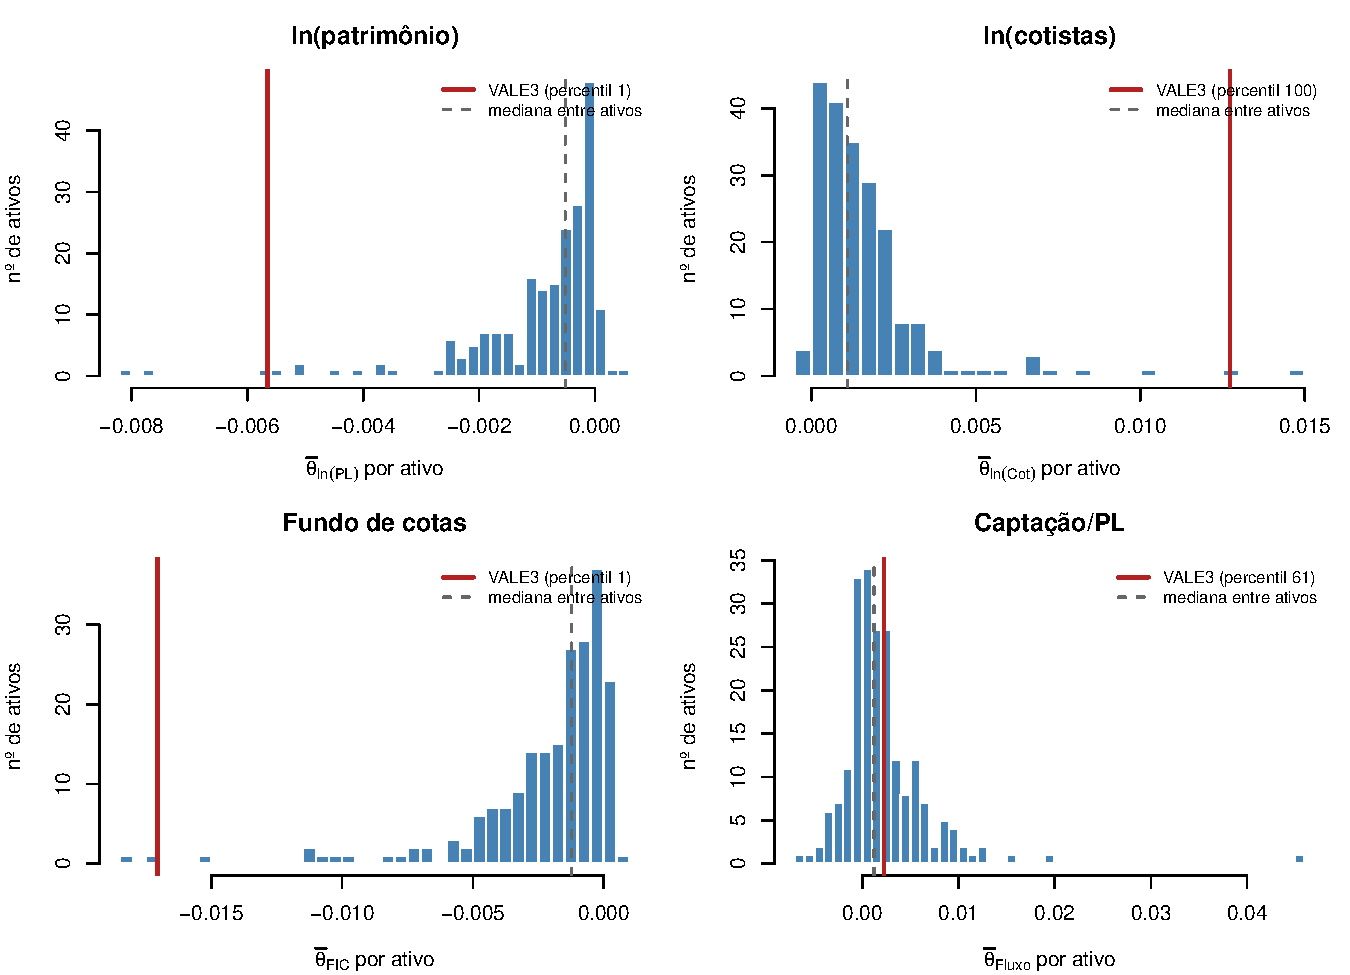
\includegraphics[width=0.85\textwidth]{fig_multiativo_dist.pdf}
\caption{A distribuição dos coeficientes entre os 207 ativos, com VALE3 marcado em vermelho ---
repare como ele fica na cauda em três dos quatro painéis.}
\end{figure}

\subsubsection*{Um detalhe técnico da regressão que soma todos os ativos numa conta só}

A Seção 5.3 do \texttt{tcc I.pdf} traz uma checagem complementar, empilhando todas as observações
de todos os ativos numa única regressão, com um ``efeito-fixo de ativo e de mês''. Isso é feito por
uma técnica chamada \textbf{demeaning iterativo} (ou Frisch--Waugh--Lovell): em vez de criar uma
coluna extra na regressão para cada um dos 444 ativos e cada um dos 72 meses (o que seria
tecnicamente equivalente, mas pesado demais para calcular), o método subtrai repetidamente a média
de cada ativo e a média de cada mês, até os números pararem de mudar. \analogia{É parecido com
tirar o ``sabor de cada tempero'' de uma receita, subtraindo a média de cada ingrediente
repetidamente, até sobrar só o ``sabor combinado'' que você quer estudar, sem nenhum ingrediente
específico dominando a conta.} O resultado confirma os mesmos três sinais estruturais, agora numa
única regressão com quase 900 mil observações.

% ======================================================================
\section{Juntando tudo: a história completa, em um parágrafo}

As características de um fundo (tamanho, cotistas, tipo) explicam bem o peso de VALE3 que ele
carrega, com sinais estáveis por 72 meses e que generalizam para um universo amplo de outras
ações (embora VALE3, em magnitude, seja um caso extremo, não típico) --- isso é a Parte 1 do
trabalho, resolvida com Fama--MacBeth, Newey--West e o modelo logístico, e reforçada pela margem
extensiva: fundos grandes e de cotas são mais propensos a \emph{ter} VALE3, mas carregam
\emph{menos} dela, a assinatura de diversificação. Só que essas mesmas características
\textbf{não ajudam a prever} a mudança de peso de um mês para o outro --- o peso se comporta
quase como um passeio aleatório no curto prazo (confirmado pelo teste de Dickey--Fuller: os
fatores revertem à média, mas devagar), e nenhum dos modelos estruturais bate a simples previsão
de repetir o último valor. Ainda assim, existe uma reversão real, porém lenta, ao peso que as
características sugerem --- o modelo de ajuste parcial mede essa velocidade, com quatro métodos
diferentes que concordam no sinal (exceto o Arellano-Bond, que não se comporta bem nesse formato
específico de painel) uma vez corrigido o erro-padrão pelo efeito de tempo, mas discordam
bastante na magnitude, revelando que parte dos fundos se ajusta rápido (dentro da própria
trajetória) e parte carrega um desvio permanente que nunca fecha. E mesmo essa reversão, testada
formalmente pelo teste de Diebold--Mariano, só bate a previsão ingênua com confiança estatística
no horizonte que não é operável na prática --- a história tem um final honesto, não um final
triunfante.

\end{document}
